%% Included in decks: slidemage-manual, slidemage-manual-copy
%%

% SlideMage manual, chapter "Working in SlideMage": the command palette
% (tools/manual/make_screenshots.py, shot palette-search).
\setSlideVersion{1-0-0}
\begin{standardframe}{Find anything}
	\small
	One search box reaches every command, every slide and every file of the project: press \SMCode{Ctrl+K} (or \SMCode{Ctrl+Shift+F}) anywhere in the workspace.
	\par\medskip
	\begin{columns}[T,onlytextwidth]
		\begin{column}{0.54\linewidth}
			{\setlength{\fboxsep}{0pt}\fcolorbox{c_primary_gray}{white}{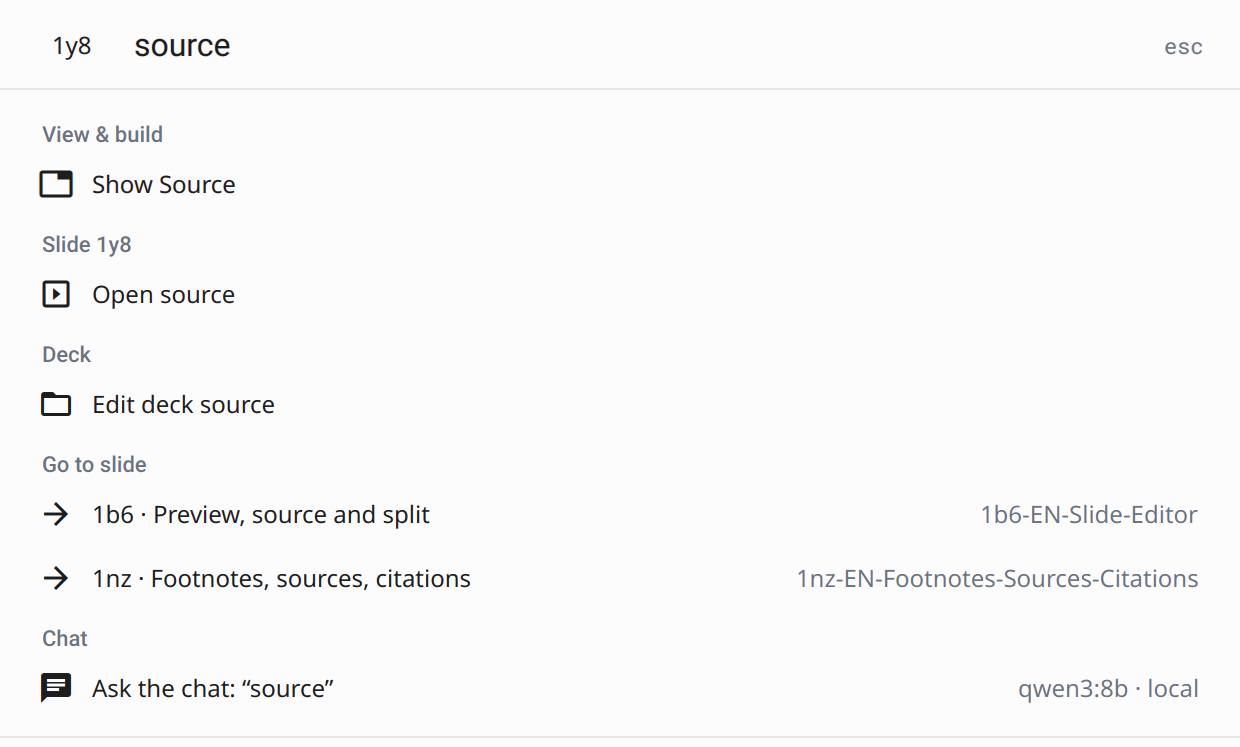
\includegraphics[width=\dimexpr\linewidth-0.8pt\relax]{media/screenshot-slidemage-palette.png}}}
		\end{column}
		\begin{column}{0.43\linewidth}
			\shrinklists{2}
			\begin{itemize}
				\item Type to filter: commands (\emph{View \& build}, \emph{Slide}, \emph{Deck}, \emph{Project}), slides to go to, and, from three characters on, text in slides, deck files and the bibliography
				\item \SMCode{Up} and \SMCode{Down} move, \SMCode{Enter} runs, \SMCode{Esc} closes
				\item Empty, it lists all commands, each with its shortcut: whatever the menus offer is here too
				\item \emph{Ask the chat} sends your text to the assistant
			\end{itemize}
		\end{column}
	\end{columns}
\end{standardframe}
